% Fairmeta showcase preprint; build via ./compile_main.sh
\documentclass[twocolumn]{fairmeta}
% Packages for paper/main.tex (fairmeta). fairmeta.cls already loads graphicx,
% booktabs, bm, hyperref, natbib, subcaption, xcolor, tikz (via tcolorbox), etc.
\usepackage{amsmath}
% Times text + matching math (heavier strokes than Computer Modern; common in ML journal PDFs).
% Omit amssymb/amsfonts: newtxmath supplies AMS-compatible symbols.
\usepackage{newtxtext,newtxmath}
% Full-width displays in \texttt{twocolumn} (e.g.\ key equations).
\usepackage{cuted}
\usepackage{tabularx}
\usepackage{url}
\usepackage{listings}
\usepackage{tikz}
\usetikzlibrary{arrows.meta, calc, positioning, shapes.geometric, decorations.pathreplacing, backgrounds}
\usepackage{algorithm}
\usepackage{algpseudocode}
\usepackage{pgfplots}
\pgfplotsset{compat=1.18}
\usepackage{chemformula}
\usepackage[version=4]{mhchem}
\usepackage{float}
\usepackage{textcomp}

\usepackage[most]{tcolorbox}
\newtcolorbox{agentthought}{
  colback=activepurple!8, colframe=activepurple!60,
  fonttitle=\small\sffamily\bfseries, title={Agent thought ($t_i$)},
  boxrule=0.4pt, arc=2pt, left=4pt, right=4pt, top=2pt, bottom=2pt,
  before skip=4pt, after skip=4pt
}
\newtcolorbox{toolcall}[1][]{
  colback=ragblue!8, colframe=ragblue!60,
  fonttitle=\small\sffamily\bfseries, title={#1},
  boxrule=0.4pt, arc=2pt, left=4pt, right=4pt, top=2pt, bottom=2pt,
  before skip=4pt, after skip=4pt
}
\newtcolorbox{observation}{
  colback=psmilesgreen!8, colframe=psmilesgreen!60,
  fonttitle=\small\sffamily\bfseries, title={Observation ($o_i$)},
  boxrule=0.4pt, arc=2pt, left=4pt, right=4pt, top=2pt, bottom=2pt,
  before skip=4pt, after skip=4pt
}

\definecolor{deepblue}{RGB}{0,0,120}
\definecolor{midgreen}{RGB}{0,120,0}
\definecolor{darkred}{RGB}{120,0,0}
\definecolor{codecolor}{RGB}{240,240,240}
\definecolor{ragblue}{RGB}{51,122,183}
\definecolor{psmilesgreen}{RGB}{92,184,92}
\definecolor{mdorange}{RGB}{240,173,78}
\definecolor{activepurple}{RGB}{150,100,200}
\definecolor{expbteal}{RGB}{0,128,128}
\definecolor{expccopper}{RGB}{180,90,40}

% Section hierarchy: slightly denser than fairmeta defaults but not flat (reads closer to ML journal prose)
\titleformat{\section}{\large\sffamily\bfseries}{\thesection}{0.5em}{}
\titleformat{\subsection}{\normalsize\sffamily\bfseries}{\thesubsection}{0.5em}{}
\titleformat{\subsubsection}{\normalsize\sffamily\bfseries}{\thesubsubsection}{0.5em}{}
\titlespacing*{\section}{0pt}{0.85ex plus 0.2ex minus 0.1ex}{0.35ex plus 0.1ex}
\titlespacing*{\subsection}{0pt}{0.7ex plus 0.15ex}{0.3ex plus 0.1ex}
\titlespacing*{\subsubsection}{0pt}{0.6ex plus 0.1ex}{0.28ex plus 0.05ex}

\lstset{
  backgroundcolor=\color{codecolor},
  basicstyle=\tiny\ttfamily,
  keywordstyle=\color{deepblue},
  commentstyle=\color{midgreen},
  stringstyle=\color{darkred},
  showstringspaces=false,
  breaklines=true,
  frame=single,
  captionpos=b,
  numbers=left,
  numberstyle=\tiny\color{gray}
}


\title{Biologics AI: End-to-End Polymer Excipient Discovery with Agent-Backed Retrosynthesis}

\author[1]{Otun Martins}
\affiliation[1]{Algonix Ltd., United Kingdom}
\metadata[Domain]{\href{https://algonix.co.uk}{algonix.co.uk}}
\metadata[Code]{\url{https://github.com/otunmartins/insulin-ai}}
\correspondence{O.M. (\email{martins@algonix.co.uk})}

\abstract{%
Protein biologics require excipients that stabilize the active ingredient at ambient temperature, yet the combinatorial polymer design space is too large for exhaustive experiment and synthesis routes are rarely checked at discovery time.
Building on our physics-grounded agentic framework~\cite{martins2026insulin}, we generalize the MCP orchestration layer to any biologic target and integrate agent-backed macromolecular retrosynthesis, a four-tier precursor registry, and regulatory screening as default stages in every human-in-the-loop iteration.
Two independent five-iteration campaigns on insulin (PDB 4F1C) and adalimumab (PDB 3WD5) ran the same workflow unchanged across targets.
The insulin session converged on poly(carbonate-alt-lactide) at $-1787.6$~kJ/mol ($2.69\times$ PEG within the session), where lactate ester comonomers add bidentate carbonyl hydrogen-bonding to a carbonate backbone.
The adalimumab session reached poly(amide-ketone) at $-3337.1$~kJ/mol (discovery score 64.24) with a succinimide ring-opening route; bulky copolymer designs failed Packmol packing while a simple ketone--amide linear backbone packed and scored best.
Head-to-head comparisons against reinforcement learning and Bayesian optimization appear in our companion benchmark preprint~\cite{martins2026insulin}.}

\begin{document}
\maketitle

%% =====================================================================
\section{Introduction}
%% =====================================================================

Monoclonal antibodies, enzymes, peptides, and other biologics share a formulation problem with insulin: the combinatorial space of polymer excipients is vast, and candidate materials must both stabilize the protein and be synthesizable at scale~\cite{hsu2022glycosylated}.
Cold-chain dependence limits access in resource-limited settings; a thermally protective matrix polymer could change that calculus, but no single experimental campaign can screen more than a tiny fraction of chemically plausible repeat units while also checking residual-monomer safety and synthetic feasibility.

Our prior work~\cite{martins2026insulin} established a physics-grounded agentic loop for insulin in which a large language model (LLM) calls OpenMM Packmol-matrix screening through the Model Context Protocol (MCP)~\cite{mcp2024}, maintains a persistent discovery world, and was benchmarked against reinforcement learning and tree-structured Parzen optimization under matched oracle budgets.
That manuscript fixed the protein target to insulin and treated synthesis planning as out of scope.
Readers who want regret curves and baseline comparisons against DQN, PPO, and Optuna should consult that preprint; the present work asks a complementary question: can the same architecture run end to end for \emph{any} biologic, with retrosynthesis and regulatory screening closed before each iteration checkpoint?

We answer by documenting the generalized Biologics AI workflow and by walking through two showcase campaigns.
The MCP server now resolves arbitrary biologic names or PDB identifiers, writes retrosynthesis plans from agent-supplied literature extractions (not from a second LLM inside RetroSynAgent), seeds knowledge-graph trees from a four-tier precursor registry, and records ADMET, excipient compliance, and audit artifacts alongside OpenMM structure files.
Each campaign ran for five human-in-the-loop (HITL) iterations with mandatory Step~7 checkpoints; within-session progression, structure--activity relationships, and synthesis routes are the primary readouts.

Three extensions distinguish this work from~\cite{martins2026insulin}.
We first describe biologic-agnostic orchestration via \texttt{resolve\_biologic\_target} and parameterized Packmol-matrix screening (\S\ref{sec:biologic}).
We second document the retrosynthesis subsystem that was engineered so macromolecular routes close reliably: agent-as-extractor JSON, diagnose/register retry, session precursor seeding, and hang guards (\S\ref{sec:retro}).
We third present dual showcase campaigns on insulin and adalimumab (\S\S\ref{sec:insulin}--\ref{sec:adalimumab}), including PyMOL-style complex renderings of polymer shells around each target protein (Figure~\ref{fig:showcase_chemviz}).

%% =====================================================================
\section{Platform overview}
\label{sec:platform}
%% =====================================================================

\subsection{Platform architecture}

We implement the workflow as a single Python MCP server (FastMCP) that registers tools for biologic resolution, literature mining, polymer validation, molecular screening, cheminformatics mutation, retrosynthesis, ADMET, excipient compliance, and session management.
It runs inside the \texttt{biologix-ai-sim} conda environment, which bundles OpenMM~\cite{eastman2017openmm}, RDKit~\cite{landrum2013rdkit}, Packmol~\cite{packmol2009}, the Open Force Field toolkit~\cite{qiu2021development}, and RetroSynAgent dependencies.
An LLM hosted by OpenCode (or Cursor) connects to this server and calls tools in response to user prompts; model weights, tool schema, and session artifacts are version-controlled alongside the scientific code.

Figure~\ref{fig:architecture} summarizes the data flow, extending the architecture diagram of~\cite{martins2026insulin} with biologic resolution, retrosynthesis, safety screening, and iteration checkpoints.
The pipeline consists of four horizontal layers: discovery (literature, PSMILES, OpenMM), retrosynthesis closure, regulatory screening, and session state.
Each discovery session creates a folder under \texttt{runs/<session\_id>/} containing per-iteration state files (\texttt{agent\_iteration\_N.json}), a structured world-model rollup (\texttt{discovery\_world.json}), cumulative best-candidate records, minimized complex PDBs and preview PNGs under \texttt{structures/}, retrosynthesis plans (\texttt{retrosynthesis/plan\_*.json}, \texttt{llm\_res.json}), pipeline audit entries, checkpoints (\texttt{checkpoints/post\_iteration\_N.json}), and a compiled summary report (Markdown and PDF).
These artifacts let a reader reconstruct both the numerical rankings and the three-dimensional packing geometry that produced them.

\begin{figure*}[!t]
\centering
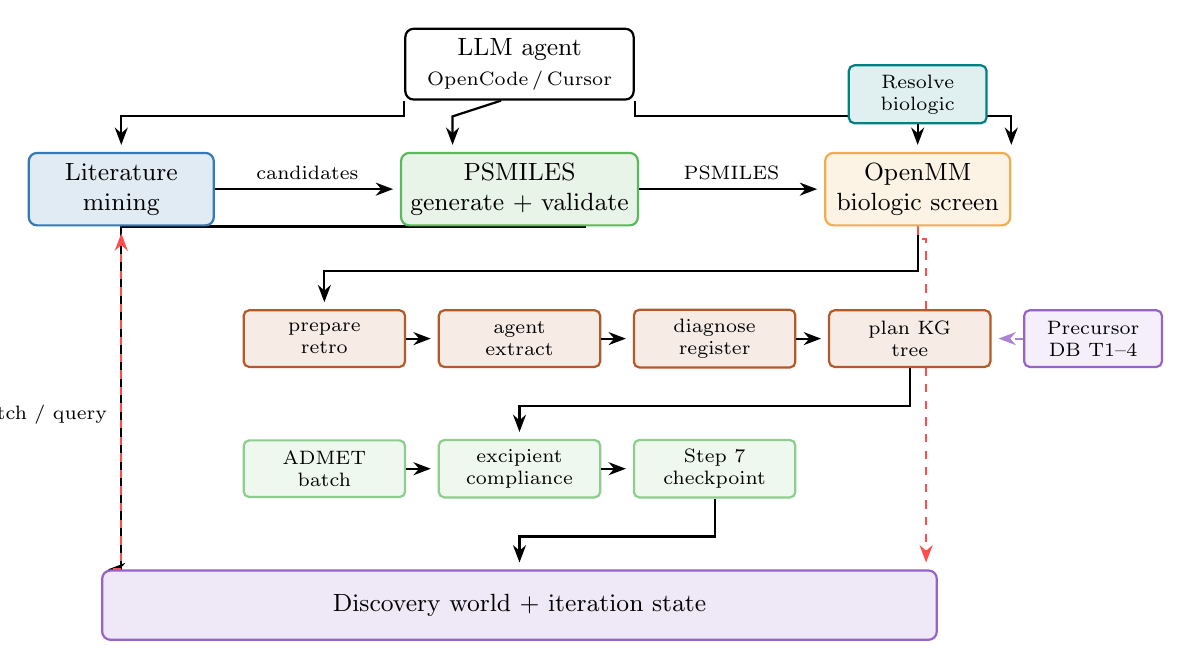
\begin{tikzpicture}[
    font=\small,
    node distance=0.50cm and 0.40cm,
    box/.style={rectangle, rounded corners=3pt, draw, thick,
                minimum width=2.35cm, minimum height=0.92cm, align=center},
    smbox/.style={rectangle, rounded corners=2pt, draw, thick,
                  minimum width=2.05cm, minimum height=0.72cm, align=center, font=\scriptsize},
    litbox/.style={box, fill=ragblue!15, draw=ragblue, fill opacity=1},
    genbox/.style={box, fill=psmilesgreen!15, draw=psmilesgreen, fill opacity=1},
    simbox/.style={box, fill=mdorange!15, draw=mdorange, fill opacity=1},
    biobox/.style={smbox, fill=expbteal!12, draw=expbteal, minimum width=1.75cm, fill opacity=1},
    retrobox/.style={smbox, fill=expccopper!12, draw=expccopper, fill opacity=1},
    safebox/.style={smbox, fill=psmilesgreen!10, draw=psmilesgreen!70, fill opacity=1},
    sidebox/.style={smbox, fill=activepurple!10, draw=activepurple, minimum width=1.75cm, fill opacity=1},
    statebox/.style={box, fill=activepurple!15, draw=activepurple,
                     minimum width=10.6cm, minimum height=0.88cm, fill opacity=1},
    topbox/.style={box, fill=white, minimum width=2.9cm, minimum height=0.88cm, fill opacity=1},
    arr/.style={-{Stealth[length=2.2mm]}, thick, shorten >=2.5pt},
    fb/.style={arr, dashed, color=red!70},
    darr/.style={arr, dashed, color=activepurple!80},
    lbl/.style={font=\scriptsize, inner sep=1pt, fill=white, fill opacity=0.92, text opacity=1}
]
% Row 1 (top): LLM agent
\node[genbox] (gen) {PSMILES\\generate + validate};
\node[litbox, left=2.35cm of gen] (lit) {Literature\\mining};
\node[simbox, right=2.35cm of gen] (sim) {OpenMM\\biologic screen};
\node[topbox, above=0.65cm of gen] (llm) {LLM agent\\{\scriptsize OpenCode\,/\,Cursor}};
\node[biobox, above=0.35cm of sim] (bio) {Resolve\\biologic};

% Row 2: retrosynthesis pipeline (centered under discovery row)
\node[retrobox, below=1.05cm of gen] (rextr) {agent\\extract};
\node[retrobox, left=of rextr] (rprep) {prepare\\retro};
\node[retrobox, right=of rextr] (rdiag) {diagnose\\register};
\node[retrobox, right=of rdiag] (rplan) {plan KG\\tree};
\node[sidebox, right=of rplan] (prec) {Precursor\\DB T1--4};

% Row 3: safety screening
\node[safebox, below=0.90cm of rextr] (comp) {excipient\\compliance};
\node[safebox, left=of comp] (admet) {ADMET\\batch};
\node[safebox, right=of comp] (chk) {Step 7\\checkpoint};

% Row 4 (bottom): discovery world (span matches retro row, not outer-gutter rails)
\node[statebox, below=0.90cm of comp] (world) {Discovery world + iteration state};

% Clip TeX bounding box to diagram content (no outer-gutter overflow into margins)
\useasboundingbox ([xshift=0.04cm]lit.west |- llm.north) rectangle ([xshift=-0.04cm]prec.east |- world.south);

% Attachment points (avoid vertical spine through labels)
\coordinate (genTopIn) at ($(gen.north west)!0.22!(gen.north east)$);
\coordinate (genBotOut) at ($(gen.south west)!0.78!(gen.south east)$);

% Inter-row buses: strictly between row bottoms/tops (inside diagram width)
\coordinate (busLLMDisc) at ([yshift=-0.20cm]llm.south);
\coordinate (busDiscRetro) at ($([yshift=-0.12cm]gen.south)!0.55!([yshift=0.12cm]rprep.north)$);
\coordinate (busRetroSafe) at ($([yshift=-0.12cm]rprep.south)!0.55!([yshift=0.12cm]comp.north)$);
\coordinate (busSafeWorld) at ($([yshift=-0.12cm]admet.south)!0.55!([yshift=0.12cm]world.north)$);

% Discovery pipeline (horizontal, mid-row)
\draw[arr] (lit.east) -- (gen.west) node[lbl, midway, above=2pt] {candidates};
\draw[arr] (gen.east) -- (sim.west) node[lbl, midway, above=2pt] {PSMILES};
\draw[arr] (bio.south) -- (sim.north);

% Connectors behind boxes: horizontals only in inter-row gutters (no rails outside lit/prec)
\begin{scope}[on background layer]
  % LLM fan-out via bus just below agent (sim enters at north east, clear of Resolve biologic)
  \draw[arr] (llm.south west) -- (llm.south west |- busLLMDisc)
    -- (lit.north |- busLLMDisc) -- (lit.north);
  \draw[arr] ($(llm.south west)!0.42!(llm.south east)$)
    -- ($(llm.south west)!0.42!(llm.south east)$ |- busLLMDisc)
    -- (genTopIn |- busLLMDisc) -- (genTopIn);
  \draw[arr] (llm.south east) -- (llm.south east |- busLLMDisc)
    -- (sim.north east |- busLLMDisc) -- (sim.north east);
  % Inter-row buses (stay within [lit.west, prec.east]; shafts render behind boxes)
  \draw[arr] (sim.south) -- (sim.south |- busDiscRetro)
    -- (rprep.north |- busDiscRetro) -- (rprep.north);
  \draw[arr] (rplan.south) -- (rplan.south |- busRetroSafe)
    -- (comp.north |- busRetroSafe) -- (comp.north);
  \draw[arr] (chk.south) -- (chk.south |- busSafeWorld)
    -- (world.north |- busSafeWorld) -- (world.north);
  % PSMILES -> world via Literature column (avoids rextr/comp under gen; stays in bounds)
  \draw[arr] (genBotOut) -- (genBotOut -| lit.south)
    -- (lit.south |- world.north west) -- (world.north west);
  % Feedback (short corner drops; matched left/right symmetry, as in [14])
  \draw[fb] (sim.south) -- ++(0,-0.16) -| ($(world.north east)+(-0.15,0)$);
  \draw[fb] ($(world.north west)+(0.15,0)$) -| (lit.south);
\end{scope}
\node[lbl, anchor=east, xshift=-4pt]
  at ($(lit.south)!0.55!(lit.south |- world.north west)$) {patch / query};

% Intra-row pipeline (foreground; arrows between adjacent boxes only)
\draw[arr] (rprep.east) -- (rextr.west);
\draw[arr] (rextr.east) -- (rdiag.west);
\draw[arr] (rdiag.east) -- (rplan.west);
\draw[darr] (prec.west) -- (rplan.east);
\draw[arr] (admet.east) -- (comp.west);
\draw[arr] (comp.east) -- (chk.west);
\end{tikzpicture}
\caption{Platform architecture (extended from~\cite{martins2026insulin}).
Solid arrows denote MCP tool calls from the LLM agent; dashed arrows show feedback through session state.
Rows~2--3 run for OpenMM pass candidates each iteration.
The retrosynthesis branch closes synthesis feasibility; the precursor registry supplies leaf coverage for the knowledge-graph tree.}
\label{fig:architecture}
\end{figure*}

\subsection{Probabilistic chain formalism}
\label{sec:formalism}

As in our prior work~\cite{martins2026insulin}, we model the discovery loop as a probabilistic chain over tool calls~\cite{stephens2025mathframing}.
Given an initial context $c$ (user objective, tool schema, and seed state), the probability of executing an action sequence $\mathbf{a} = (a_1, \ldots, a_n)$ is
\begin{equation}
P(\mathbf{a} \mid c) = \prod_{i=1}^{n} P(a_i \mid s_{i-1},\, c),
\label{eq:chain}
\end{equation}
where $s_0 = s_0(c)$ is the initial prompt state and $s_i = u(a_i, s_{i-1})$ is the state update~\cite{puterman1994mdp}.
Under the ReAct formalism the LLM generates a reasoning trace (``thought'') $t_i$ before each tool call, so
\begin{equation}
P^t(a_i \mid s_{i-1}) = P(a_i \mid t_i, s_{i-1})\; P(t_i \mid s_{i-1}).
\label{eq:react}
\end{equation}
Each action decomposes as $a_i \to (\alpha_i, x_i, o_i)$, where $\alpha_i$ is an MCP tool class, $x_i$ is its argument, and $o_i$ is the returned observation.
The extended platform adds tool classes beyond~\cite{martins2026insulin}: biologic resolution, retrosynthesis (prepare, submit, diagnose, plan), ADMET, compliance, checkpoint, and world patching.

The screening oracle $f\!:\!\mathcal{X}\!\to\!\mathbb{R}$ returns the biologic--polymer interaction energy,
\begin{equation}
f(x) = E_\text{int}(x) + \epsilon, \quad \epsilon \sim \mathcal{N}(0,\,\sigma^2),
\label{eq:oracle}
\end{equation}
where $\mathcal{X}$ is the discrete space of valid PSMILES and $\sigma$ captures stochastic packing variability (${\sim}$15\% in our protocol~\cite{martins2026insulin}).

\subsection{Biologic resolution}
\label{sec:biologic}

Before screening, the agent calls \texttt{resolve\_biologic\_target(name\_or\_pdb\_id, fetch\_pdb=true)}.
The service maps common biologic names to PDB identifiers (e.g.\ insulin $\to$ 4F1C, adalimumab $\to$ 3WD5), fetches or caches the structure, and sets \texttt{BIOLOGIX\_AI\_TARGET\_PROTEIN\_PDB} for the OpenMM oracle.
The same Packmol-matrix protocol described in~\cite{martins2026insulin} then packs polymer oligomers around the resolved protein; only the PDB path and session metadata change between campaigns.

\subsection{Discovery world model}

Inspired by the structured world model in Kosmos~\cite{kosmos2025}, we maintain a session-scoped JSON document (\texttt{discovery\_world.json}) that accumulates:
\begin{itemize}
\item \textbf{Objective and history:} the user's research goal and mid-campaign steering notes.
\item \textbf{Literature entries:} stable IDs, titles, one-sentence claims, source iteration, and optional DOI or Semantic Scholar identifiers.
\item \textbf{Simulation entries:} PSMILES, interaction energy, screening status, and pointers to structure artifacts; may link to \texttt{retrosynthesis/plan\_*.json}.
\item \textbf{Hypotheses:} free-text statements with supporting evidence IDs and a status tag (open, supported, weak, dropped); may cite blocking reactants from retrosynthesis diagnosis.
\item \textbf{Open questions and human directives:} recorded per iteration for traceability.
\end{itemize}
Three MCP tools operate on this file: \texttt{patch\_discovery\_world}, \texttt{discovery\_world\_planning\_context}, and \texttt{get\_discovery\_world\_state}.
When the agent calls \texttt{save\_discovery\_state} after each iteration, the server updates \texttt{meta.last\_iteration} and links the latest \texttt{agent\_iteration\_N.json} into the world file.

\subsection{Extended agentic discovery loop}
\label{sec:loop}

A single HITL iteration follows the seven-step protocol in \texttt{biologics-delivery-discovery.md}:
\begin{enumerate}
\item \textbf{Literature mining.} Adaptive Semantic Scholar~\cite{lo2020s2orc} queries from hypotheses, open questions, and prior top performers.
\item \textbf{Candidate generation.} Material names convert to PSMILES via a curated polymer lookup with PubChem fallback; RDKit validation enforces exactly two \texttt{[*]} connection points.
\item \textbf{OpenMM screening.} Validated PSMILES are evaluated by the Packmol-matrix protocol against the resolved biologic structure.
\item \textbf{Retrosynthesis.} For each pass candidate: \texttt{prepare\_retrosynthesis} $\to$ agent extraction JSON $\to$ \texttt{submit\_retro\_extractions} $\to$ optional \texttt{diagnose\_retro\_extractions} / \texttt{register\_retro\_precursors} $\to$ \texttt{plan\_retrosynthesis}.
\item \textbf{Monomer ADMET.} \texttt{check\_monomers\_batch} on plan monomers.
\item \textbf{Excipient compliance.} \texttt{check\_excipient\_compliance} against FDA/EMA/GRAS rules and immunogenicity SMARTS.
\item \textbf{Iteration checkpoint.} Mandatory pause: \texttt{save\_discovery\_state}, summary report, funnel checkpoint; the agent waits for user feedback before the next iteration.
\end{enumerate}

Algorithm~\ref{alg:agentic} formalizes the loop; Algorithm~\ref{alg:retro_retry} (Appendix~\ref{app:retro}) details the diagnose/retry branch.

\begin{algorithm}[t]
\caption{Extended Agentic Discovery Loop}\label{alg:agentic}
\small
\begin{algorithmic}[1]
\Require context $c$, biologic $b$, oracle $f$, iterations $N$
\State $s_0 \gets s_0(c)$; $\mathcal{W}_0 \gets \emptyset$; $\mathcal{D}_0 \gets \emptyset$
\State $b \gets \texttt{resolve\_biologic\_target}(b)$
\For{$t = 1, \ldots, N$}
  \State $t_i \gets \text{LLM reason over } s_{t-1}$
  \State $\alpha_i \gets$ select from extended MCP tool set
  \State $o_i \gets \alpha_i(x_i)$
  \If{$\alpha_i = \texttt{screen}$}
    \State $y_t \gets f(x_i)$; $\mathcal{D}_t \gets \mathcal{D}_{t-1} \cup \{(x_i, y_t)\}$
  \ElsIf{$\alpha_i = \texttt{retro\_submit}$ \textbf{and} \texttt{blocking\_reactants} $\neq \emptyset$}
    \State retry $\gets$ \texttt{diagnose/register} (Alg.~\ref{alg:retro_retry})
  \EndIf
  \State $s_t \gets u_\text{sel}(a_i,\, s_{t-1})$; $\mathcal{W}_t \gets \texttt{patch\_world}(\mathcal{W}_{t-1},\, o_i,\, t_i)$
  \State \textbf{wait for user} at Step~7 checkpoint
\EndFor
\State \Return best $(x, y)$ in $\mathcal{D}_N$ with retro plan artifacts
\end{algorithmic}
\end{algorithm}

\subsection{Retrosynthesis subsystem and enabling modifications}
\label{sec:retro}

Macromolecular retrosynthesis runs in two stages.
In \textbf{Stage~1 (extraction)}, the OpenCode agent reads literature PDFs returned by \texttt{prepare\_retrosynthesis} and writes reaction JSON to \texttt{llm\_res.json}; RetroSynAgent's internal LLM is not used.
The agent must supply at least two reactions when polymerization reactants are not commodity chemicals (downstream polymerization plus upstream intermediate synthesis).
In \textbf{Stage~2 (KG expansion)}, \texttt{plan\_retrosynthesis} builds a RetroSynAgent~\cite{ma2025retrosynagent} knowledge-graph tree to purchasable leaves, seeded by session precursors and the bundled registry.

Table~\ref{tab:retro_stack} lists the engineering layers that make this pipeline reliable in practice.

\begin{table}[t]
\centering
\caption{Retrosynthesis stack components and their roles.}
\label{tab:retro_stack}
\small
\begin{tabularx}{\columnwidth}{lX}
\toprule
Layer & Purpose \\
\midrule
Agent as extractor & OpenCode writes \texttt{llm\_res.json}; auditable reaction text \\
Multi-step extractions & Minimum two reactions for non-commodity precursors \\
PSMILES / name bridge & \texttt{psmiles\_bridge}, \texttt{retro\_adapter}: tree root = polymer name \\
Tier 1--4 precursor DB & Manual JSON, SMiPoly, Molport InChIKeys, ZINC HDF5 \\
Session seeding & \texttt{seed\_workspace\_precursors} before \texttt{Tree.construct\_tree()} \\
Diagnose / register MCP & Retry when \texttt{kg\_empty\_after\_session\_extractions} \\
Bootstrap patch & Extended \texttt{CommonSubstanceDB}; timed PubChem wrapper \\
Hang prevention & PDF subprocess timeout, tree timeout, PSMILES/CTA guards \\
Agent CTA rules & Reagents registered via \texttt{register\_retro\_precursors}, not as retro targets \\
Provenance honesty & \texttt{session\_agent\_llm} metadata; no invented routes \\
\bottomrule
\end{tabularx}
\end{table}

\begin{table}[t]
\centering
\caption{Precursor registry tiers (built by \texttt{scripts/build\_precursor\_db.py}).}
\label{tab:precursor_tiers}
\scriptsize
\setlength{\tabcolsep}{3pt}
\begin{tabularx}{\columnwidth}{clXl}
\toprule
Tier & Source & Scale & Runtime role \\
\midrule
1 & \texttt{precursors.json} & ${\sim}$244 entries & Specialty monomers \\
2 & SMiPoly CSV & ${\sim}$1k & Polymer monomers \\
3 & Molport & ${\sim}$997k InChIKeys & Building-block bridge \\
4 & ZINC stock & ${\sim}$17M InChIKeys & Purchasable leaves \\
\bottomrule
\end{tabularx}
\end{table}

When \texttt{submit\_retro\_extractions} returns non-empty \texttt{blocking\_reactants}, the agent calls \texttt{diagnose\_retro\_extractions}, then either \texttt{register\_retro\_precursors} for commercially available specialty reagents or expands upstream reactions and re-submits (maximum two retries).

\paragraph{Extraction quality and provenance tracking.}
A distinctive feature of this retrosynthesis architecture is that the LLM agent---not a second model inside RetroSynAgent---performs reaction extraction from literature.
This design choice has three consequences.
First, extraction quality depends on the agent's chemical reasoning rather than a purpose-trained reaction extraction model; the agent may propose mechanistically analogous routes that lack direct precedent (see \S\ref{sec:adalimumab} for an example).
Second, provenance is explicit: every route carries a \texttt{session\_agent\_llm} tag that distinguishes agent-proposed chemistry from database-backed reactions (AiZynthFinder or template routes).
Third, the multi-step extraction requirement (minimum two reactions for non-commodity precursors) forces the agent to reason about upstream intermediates, not merely name a polymer and a monomer.

The knowledge-graph tree built by \texttt{plan\_retrosynthesis} succeeds when all leaf nodes resolve to Tier~1--4 precursors.
Failure modes include: (a)~blocking reactants not in any tier, triggering the diagnose/register loop; (b)~PSMILES targets that the PSMILES/name bridge cannot resolve, causing tree construction to abort; and (c)~agent-supplied reactions with incorrect stoichiometry or implausible conditions, which pass tree construction but require human review at Step~7.
Mode~(c) is the most insidious because the pipeline cannot detect it automatically; provenance metadata and the critical assessment paragraphs in \S\S\ref{sec:insulin}--\ref{sec:adalimumab} exist precisely to flag such cases for the human reviewer.

\subsection{Molecular screening protocol}
\label{sec:screening}

The screening objective is the non-bonded interaction energy between the target biologic and a polymer shell, following the Packmol-matrix protocol of~\cite{martins2026insulin}.
For each candidate PSMILES, the server generates a 3D oligomer conformer, packs multiple polymer chains around the resolved protein structure with Packmol~\cite{packmol2009}, assigns GAFF2/OpenFF parameters to the polymer and AMBER ff14SB to the protein~\cite{he2020amber,maier2015ff14sb,qiu2021development}, and energy-minimizes the composite.
The resulting geometry is a dense matrix in which short oligomers encircle the protein surface; representative minimized complexes from both showcase campaigns appear in Figure~\ref{fig:showcase_chemviz} (\S\ref{sec:insulin}).
The interaction energy is
\begin{equation}
E_\text{int} = E_\text{complex} - E_\text{protein} - E_\text{polymer},
\label{eq:eint}
\end{equation}
where each term is the potential energy of the specified subsystem after minimization.
More negative values indicate stronger biologic--polymer attraction.
Candidates that fail RDKit parsing, violate prescreen chemistry rules, or exceed Packmol packing timeouts are logged with verbatim failure reasons and excluded from energy rankings.

\subsection{Hang prevention and timeouts}

Retrosynthesis and literature download can stall on invalid targets or network calls.
We added bounded timeouts: PDF download subprocess (60\,s), \texttt{Tree.construct\_tree()} (120\,s), pre-flight PSMILES guards rejecting wildcard-only targets, and an 8\,s PubChem wrapper in \texttt{retrosyn\_bootstrap}.
These guards are covered by \texttt{tests/test\_retro\_hang\_guards.py} and prevent Selenium or scholarly stalls from blocking HITL sessions.

%% =====================================================================
\section{Showcase: Insulin campaign}
\label{sec:insulin}
%% =====================================================================

Session \texttt{insulin-stabilize-iter1} targeted insulin stabilization (PDB 4F1C) over five HITL iterations.
Table~\ref{tab:insulin_strategy} summarizes the iteration strategy; discovery score progressed 6.2 $\to$ 17.3 $\to$ 30.1 $\to$ 35.9 $\to$ 30.8.
Iteration~1 mined literature candidates (PEG, PLA, PLGA, chitosan, PCL) and established PEG at $-611.9$~kJ/mol as the within-session reference.
Iteration~2 applied feedback-guided mutation and discovered poly(carbonate) at $-1135.0$~kJ/mol, the first family to exceed $-900$~kJ/mol.
Iterations~3--5 expanded polycarbonate variants, then carbonate--ester hybrids, then rational linker variants guided by the Iteration~4 SAR.

\begin{table}[t]
\centering
\caption{Insulin campaign iteration strategy (\texttt{insulin-stabilize-iter1}).}
\label{tab:insulin_strategy}
\scriptsize
\setlength{\tabcolsep}{3pt}
\begin{tabularx}{\columnwidth}{clXl}
\toprule
Iter & Strategy & Evaluated & Key outcome \\
\midrule
1 & Literature mining & PEG, PLA, PLGA, chitosan, PCL & PEG bench ($-611.9$~kJ/mol) \\
2 & Feedback mutation & 8 mutants & Poly(carbonate): $-1135.0$ \\
3 & Polycarbonate expansion & 4 variants & PPC: $-1135.8$ \\
4 & Carbonate--ester hybrids & 4 designs & PC-alt-lactide: $-1787.6$ \\
5 & SAR linker variants & 6 designs & PC-alt-3HP: $-1434.0$ (new \#3) \\
\bottomrule
\end{tabularx}
\end{table}

Table~\ref{tab:insulin_ranking} lists the top candidates across all iterations (within-campaign reference: PEG at $-611.9$~kJ/mol).
The lead poly(carbonate-alt-lactide) repeat unit is shown in Figure~\ref{fig:insulin_struct}.

\begin{table*}[t]
\centering
\caption{Insulin campaign: top ten candidates by OpenMM interaction energy (within-session).}
\label{tab:insulin_ranking}
\small
\begin{tabularx}{\textwidth}{rlXlcc}
\toprule
Rank & Candidate & Iter & $E_\text{int}$ (kJ/mol) & vs PEG & Retro plan \\
\midrule
1 & Poly(carbonate-alt-lactide) & 4 & $-1787.6$ & $2.69\times$ & -- \\
2 & Hydroxy-functionalized PC & 4 & $-1699.4$ & $2.56\times$ & -- \\
3 & PC-alt-3-hydroxypropionate & 5 & $-1434.0$ & $2.34\times$ & -- \\
4 & PC-alt-2-hydroxybutyrate & 5 & $-1223.0$ & $2.00\times$ & -- \\
5 & Poly(propylene carbonate) & 3 & $-1135.8$ & $1.86\times$ & Analogous \\
6 & Poly(carbonate) & 2 & $-1135.0$ & $1.85\times$ & Complete \\
7 & PC-alt-glycerate & 5 & $-1115.1$ & $1.82\times$ & -- \\
8 & Poly(ethylene carbonate) & 3 & $-1104.6$ & $1.81\times$ & Analogous \\
9 & PC-alt-2-hydroxy-2-methylpropionate & 5 & $-1093.0$ & $1.79\times$ & -- \\
10 & Allyl-functionalized PC & 4 & $-1061.6$ & $1.60\times$ & -- \\
13 & PEG (reference) & 1 & $-611.9$ & $1.00\times$ & Complete \\
14 & PLA (reference) & 1 & $-587.3$ & $0.96\times$ & Complete \\
\bottomrule
\end{tabularx}
\end{table*}

\subsection{Structure--activity relationships}

Table~\ref{tab:insulin_sar} summarizes ester-comonomer modifications relative to the poly(carbonate) baseline at $-1135.0$~kJ/mol.
Incorporating a lactate ester segment (methyl branch plus second carbonyl) adds $-652.6$~kJ/mol, the largest single-step gain in the campaign.
The agent's Iteration~4 reasoning (Appendix~\ref{app:reasoning}) hypothesized bidentate carbonyl hydrogen-bonding: the lactate ester positions its carbonyl adjacent to the carbonate oxygen, presenting two acceptors within one repeat unit.
Hydroxymethyl substitution on the carbonate carbon adds $-564.4$~kJ/mol via an extra H-bond donor, consistent with the second-ranked hydroxy-functionalized PC at $-1699.4$~kJ/mol.
By contrast, the unsubstituted glycolate ester \emph{reduces} interaction by $+199.4$~kJ/mol relative to base carbonate, and allyl substitution adds only $+73.4$~kJ/mol, suggesting steric or conformational penalties when bulky or flexible side chains disrupt packing.

\begin{table}[H]
\centering
\caption{Insulin campaign: ester-comonomer SAR (Iteration~4--5).}
\label{tab:insulin_sar}
\scriptsize
\setlength{\tabcolsep}{2pt}
\begin{tabularx}{\columnwidth}{lccX}
\toprule
Modification & $E_\text{int}$ & $\Delta$ vs PC & Mechanism \\
\midrule
Carbonate base & $-1135.0$ & -- & C=O H-bond acceptors \\
+ Lactate ester & $-1787.6$ & $-652.6$ & Bidentate C=O + methyl \\
+ 3-Hydroxypropionate & $-1434.0$ & $-299.0$ & Longer spacer geometry \\
+ Hydroxymethyl (on C) & $-1699.4$ & $-564.4$ & OH donor \\
+ Glycolate (no branch) & $-935.6$ & $+199.4$ & Steric / flexibility penalty \\
\bottomrule
\end{tabularx}
\end{table}

Figure~\ref{fig:showcase_chemviz} (left column) shows the minimized insulin--poly(carbonate-alt-lactide) complex: polymer oligomers form a shell around the folded protein cartoon, with carbonyl-rich repeat units oriented toward the surface.
The 2D repeat unit (Figure~\ref{fig:insulin_struct}) highlights the alternating carbonate and lactate ester motif that drives the SAR above.
The Iteration~4 carbonate--ester hybrid combines a carbonate backbone ($-1135$~kJ/mol baseline) with lactate ester segments that add carbonyl hydrogen-bond acceptors and a methyl branch for hydrophobic contacts.
The agent's reasoning trace (Appendix~\ref{app:reasoning}) explicitly tied the lactate comonomer's superior performance to bidentate carbonyl geometry: two C=O acceptors within one repeat unit face the insulin surface amides (Asn, Gln, backbone NH), while the methyl branch provides a conformational lock that keeps the ester carbonyl co-planar with the carbonate oxygen.
By contrast, the glycolate ester (no branch) rotates freely, diluting surface contact and reducing interaction below the carbonate-only baseline.

\begin{figure}[H]
\centering
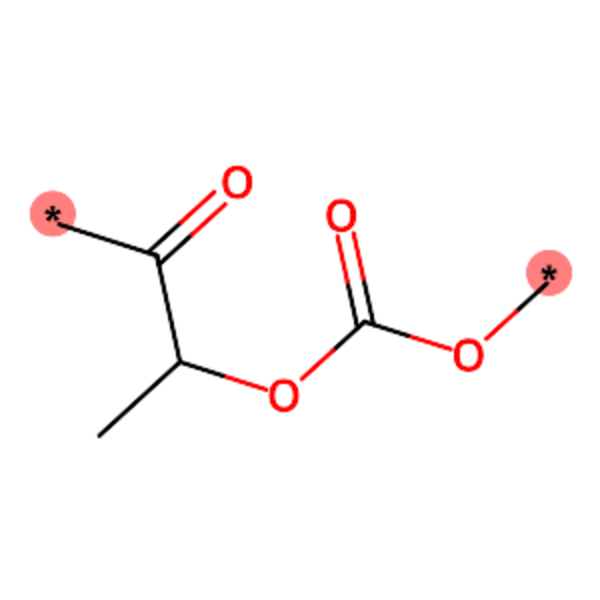
\includegraphics[width=0.72\columnwidth]{figures/insulin_pc_alt_lactide.png}
\caption{Repeat unit of poly(carbonate-alt-lactide), top insulin campaign candidate ($-1787.6$~kJ/mol).}
\label{fig:insulin_struct}
\end{figure}

Retrosynthesis for poly(carbonate) (Iteration~2) closed a three-step knowledge-graph route with \texttt{session\_agent\_llm} provenance (Table~\ref{tab:insulin_retro}).
The route proceeds from commodity CO$_2$ and ethylene oxide through cyclic carbonate intermediates to the final ring-opening polymerization (ROP) step; all leaf nodes are Tier~1--2 precursors in the bundled registry.

\begin{table}[H]
\centering
\caption{Retrosynthesis route for poly(carbonate) (insulin session, Iteration~2).}
\label{tab:insulin_retro}
\scriptsize
\begin{tabularx}{\columnwidth}{lX}
\toprule
Step & Reaction / conditions \\
\midrule
R003 & Ethylene oxide + CO$_2$ $\to$ ethylene carbonate (cycloaddition, Bu$_4$NBr, 100--150\,$^\circ$C) \\
R002 & Ethylene glycol + diphenyl carbonate $\to$ ethylene carbonate (transesterification, 120--180\,$^\circ$C) \\
R001 & Ethylene carbonate $\to$ poly(carbonate) (ROP, Sn(Oct)$_2$ or DBU, 100--160\,$^\circ$C) \\
\bottomrule
\end{tabularx}
\end{table}

\paragraph{Literature support for the polycarbonate route.}
The ring-opening copolymerization (ROCOP) of CO$_2$ and epoxides is one of the most extensively validated routes to aliphatic polycarbonates in the polymer chemistry literature.
Paul et al.~\cite{paul2015rocop} review how heterogeneous and homogeneous catalysts (Zn--Co, Cr--salen, and double metal cyanide systems) copolymerize epoxides with CO$_2$ to produce alternating polycarbonates with controlled molecular weight and narrow dispersity.
Williams and co-workers~\cite{williams2025coiii} recently demonstrated heterodinuclear Co(III)Na(I) catalysts achieving turnover frequencies $>1400$~h$^{-1}$ for propene oxide/CO$_2$ ROCOP at 20~bar and 70\,$^\circ$C, with 98\% polycarbonate selectivity.
Zhang et al.~\cite{zhang2018metalfree} confirmed that even metal-free triethylborane catalysis achieves highly alternating CO$_2$/epoxide copolymerization, validating the mechanistic feasibility of Step~R003 under mild conditions.
These references confirm that the polycarbonate retrosynthesis route extracted by the agent is chemically sound and operates under industrially accessible conditions.

For applications in drug delivery, biodegradable polycarbonates have been demonstrated as nanocarrier platforms.
Ganivada et al.~\cite{ganivada2016polycarbonate} synthesized stimuli-responsive polycarbonate--polylactide copolymers that self-assemble into tumour-targeting nanoparticles, and Arno et al.~\cite{arno2022polycarbonate} showed pH-sensitive polycarbonate graft copolymers achieving selective intracellular drug release in cancer cells.
These precedents suggest that polycarbonate backbones are compatible with biologic formulation contexts, not merely synthetic commodities.

Propylene carbonate and PEG/PLA routes from Iterations~1--3 used analogous or AiZynthFinder-informed monomer plans.
No retrosynthesis was re-run for Iteration~4 hybrids because ADMET screening returned fail disposition on monomer-level LD50 artifacts (residual monomer SMARTS, not the polymer repeat unit).

%% =====================================================================
\section{Showcase: Adalimumab campaign}
\label{sec:adalimumab}
%% =====================================================================

Session \texttt{adalimumab-stabilization-iter1} targeted adalimumab (PDB 3WD5) over five HITL iterations.
Table~\ref{tab:ada_evolution} tracks the top candidate per iteration; Iteration~5 produced the campaign best at $-3337.1$~kJ/mol.
Early iterations established PVP ($-2082.9$~kJ/mol) and the ketone-rich RND\_000 scaffold ($-2540.5$~kJ/mol at Iteration~2) as strong binders.
Iteration~4 shifted toward AlCl$_3$-free chemistry and PNIPAM ($-1590.9$~kJ/mol), a temporary regression before the Iteration~5 hybrid breakthrough.

\begin{table}[t]
\centering
\caption{Adalimumab campaign: top candidate evolution (within-session).}
\label{tab:ada_evolution}
\small
\begin{tabularx}{\columnwidth}{cXccc}
\toprule
Iter & Top candidate & $E_\text{int}$ (kJ/mol) & vs prev & Score \\
\midrule
1 & PVP & $-2082.9$ & -- & 44.16 \\
2 & RND\_000 (ketone) & $-2540.5$ & $+22\%$ & 49.99 \\
3 & RND\_000 & $-2408.4$ & $-5\%$ & 42.91 \\
4 & PNIPAM & $-1590.9$ & $-34\%$ & 30.08 \\
5 & Poly(amide-ketone) & $\mathbf{-3337.1}$ & $\mathbf{+39\%}$ & $\mathbf{64.24}$ \\
\bottomrule
\end{tabularx}
\end{table}

Iteration~5 explored eight copolymer/hybrid PSMILES combining ketone-rich (RND\_000), pyrrolidone (PVP), and amide (PNIPAM) motifs.
Seven of eight designs passed ADMET and compliance screening, but six failed Packmol packing (timeout) due to steric complexity in branched or blocky repeat units.
Only poly(amide-ketone) (\texttt{[*]CCC(=O)NC([*])=O}) completed OpenMM evaluation at $-3337.1$~kJ/mol (Figure~\ref{fig:ada_struct}).

\subsection{Packmol falsification of bulky copolymers}

The adalimumab session illustrates physics-based falsification in the same spirit as~\cite{martins2026insulin}.
Copolymer designs such as PVP-co-PNIPAM and PVP-ketone hybrids passed cheminformatics prescreening and ADMET, yet Packmol could not pack oligomers around the mAb within the timeout budget.
These failures are informative: they prune entire architectural families (blocky side chains, multiple pendant groups) before the agent spends another iteration mutating within an infeasible packing class.
Poly(amide-ketone) succeeds because its repeat unit is a simple linear chain with ketone and amide carbonyls separated by a three-carbon spacer, presenting dual hydrogen-bond acceptors without bulky pendant sterics.
Figure~\ref{fig:showcase_chemviz} (right column) shows the minimized adalimumab--poly(amide-ketone) complex; the polymer shell is visibly less congested than the failed copolymer designs would require.

\begin{figure}[H]
\centering
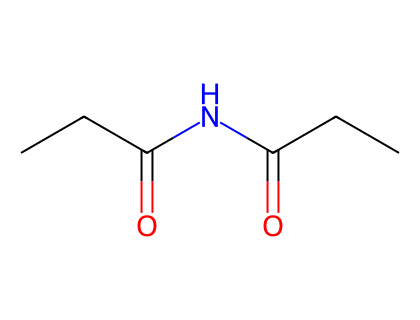
\includegraphics[width=0.72\columnwidth]{figures/adalimumab_amide_ketone.png}
\caption{Repeat unit of poly(amide-ketone), adalimumab campaign best ($-3337.1$~kJ/mol).}
\label{fig:ada_struct}
\end{figure}

Retrosynthesis closed via succinimide ring-opening polymerization (Table~\ref{tab:ada_retro}): succinic anhydride + ammonia $\to$ succinimide (commercial monomer) $\to$ poly(amide-ketone) (NaOMe catalyst, no AlCl$_3$).
Route provenance: \texttt{session\_agent\_llm}; route score 1.0.
The two-step route requires no exotic catalysts and no AlCl$_3$, addressing the Iteration~4 concern about Lewis acid residuals in pharmaceutical excipients.

\begin{table}[H]
\centering
\caption{Retrosynthesis route for poly(amide-ketone) (adalimumab session).}
\label{tab:ada_retro}
\scriptsize
\begin{tabularx}{\columnwidth}{lX}
\toprule
Step & Reaction / conditions \\
\midrule
1 & Succinic anhydride + NH$_3$ $\to$ succinimide (condensation, reflux) \\
2 & Succinimide $\to$ poly(amide-ketone) (anionic ROP, NaOMe, 180--220\,$^\circ$C) \\
\bottomrule
\end{tabularx}
\end{table}

\paragraph{Critical assessment of the succinimide route.}
The agent's proposed route merits careful scrutiny.
Succinimide (2,5-pyrrolidinedione) is a five-membered cyclic imide whose ring-opening would produce a repeat unit $-$C(=O)$-$CH$_2-$CH$_2-$C(=O)$-$NH$-$, consistent with the PSMILES \texttt{[*]CCC(=O)NC([*])=O}.
The anionic ring-opening of cyclic imides is analogous to the well-characterized anionic ring-opening of caprolactam (seven-membered cyclic amide) that produces polyamide~6~\cite{neuse2008polyaspartamides}.
However, direct anionic ROP of succinimide is uncommon in the literature; the five-membered ring is thermodynamically more stable than the seven-membered caprolactam, and the predominant industrial route to polysuccinimide proceeds instead via thermal polycondensation of L-aspartic acid at 180\,$^\circ$C under reduced pressure, retaining the cyclic imide in the backbone rather than opening it~\cite{neuse2008polyaspartamides}.
Subsequent aminolysis of polysuccinimide (ring opening with amine nucleophiles) yields polyaspartamides, a distinct polymer class.

The agent-proposed route is therefore chemically plausible by analogy with caprolactam AROP but represents a non-standard transformation that has not been experimentally demonstrated at scale for succinimide specifically.
We report the route as extracted by the agent without asserting experimental validation; the retrosynthesis subsystem records provenance (\texttt{session\_agent\_llm}) precisely so downstream experimentalists can evaluate feasibility.
This example illustrates a limitation of agent-backed retrosynthesis: the LLM extracts mechanistically analogous routes that may not have direct literature precedent for the specific monomer.

Overall campaign ranking (all iterations): (1)~poly(amide-ketone) $-3337.1$; (2)~RND\_000 $-2408.4$; (3)~PVP $-2101.6$; (4)~polycarbonate $-1752.0$; (5)~PNIPAM $-1590.9$~kJ/mol.
Absolute interaction energies are not comparable across the insulin and adalimumab proteins; within-session rankings are the intended readout.

%% =====================================================================
\section{Cross-campaign analysis}
\label{sec:cross}
%% =====================================================================

\begin{figure*}[!t]
\centering
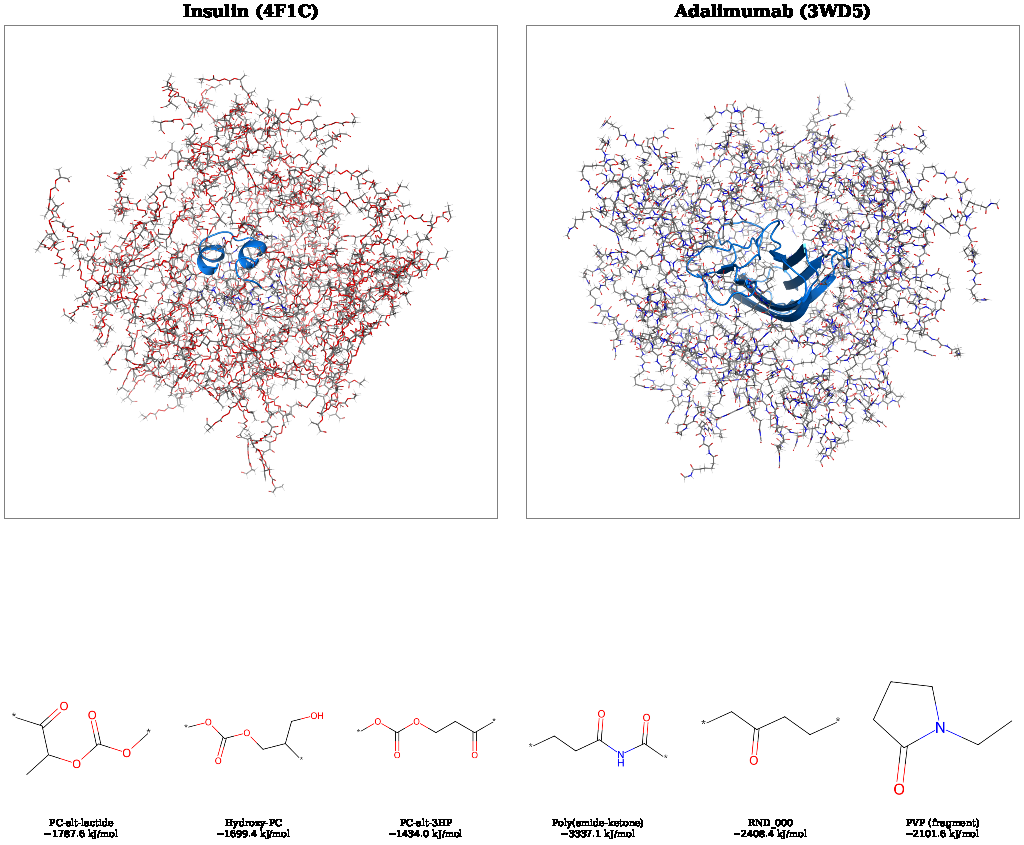
\includegraphics[width=\textwidth]{figures/showcase_chemviz_panel.pdf}
\caption{Representative polymer--biologic complexes from the showcase campaigns.
Top row: minimized Packmol-matrix geometries for the lead insulin candidate (poly(carbonate-alt-lactide), left) and adalimumab candidate (poly(amide-ketone), right); protein cartoon with DSS secondary structure, polymer ball-and-stick (PyMOL open-source, ray-traced).
Bottom row: 2D repeat units of the top three candidates per campaign, labeled with $E_\text{int}$ from the within-session ranking.}
\label{fig:showcase_chemviz}
\end{figure*}

\begin{figure}[!t]
\centering
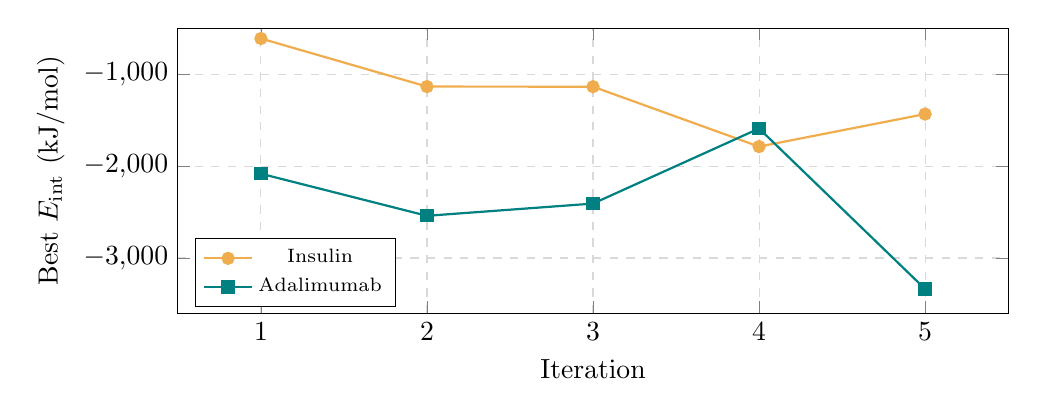
\begin{tikzpicture}
\begin{axis}[
  width=\columnwidth,
  height=5.2cm,
  xlabel={Iteration},
  ylabel={Best $E_\text{int}$ (kJ/mol)},
  legend style={font=\scriptsize, at={(0.02,0.02)}, anchor=south west},
  xmin=0.5, xmax=5.5,
  ymin=-3600, ymax=-500,
  xtick={1,2,3,4,5},
  grid=major,
  grid style={dashed,gray!30},
]
\addplot[mark=*, thick, color=mdorange] coordinates {
  (1,-612) (2,-1135) (3,-1136) (4,-1788) (5,-1434)
};
\addlegendentry{Insulin}
\addplot[mark=square*, thick, color=expbteal] coordinates {
  (1,-2083) (2,-2541) (3,-2408) (4,-1591) (5,-3337)
};
\addlegendentry{Adalimumab}
\end{axis}
\end{tikzpicture}
\caption{Best OpenMM interaction energy per iteration for insulin and adalimumab showcase campaigns.}
\label{fig:progression}
\end{figure}

Figure~\ref{fig:showcase_chemviz} presents ray-traced PyMOL renderings of the lead complexes from both campaigns; Figure~\ref{fig:progression} plots the best interaction energy per iteration for each biologic (within-campaign learning only).
Insulin shows monotonic improvement through Iteration~4 before a modest regression at Iteration~5 when the agent explored longer hydroxyalkyl spacers; adalimumab oscillates through Iteration~4 (PNIPAM dip) before the Iteration~5 poly(amide-ketone) breakthrough.

Table~\ref{tab:cross} summarizes shared workflow behavior.
Both campaigns invoked identical MCP tools and Step~7 checkpoints; only \texttt{resolve\_biologic\_target} and session metadata differed.
Despite targeting different proteins, both sessions converged on carbonyl-dense repeat units (carbonate/ester for insulin; ketone/amide for adalimumab), echoing the hydrogen-bond-dense motif convergence reported across autonomous insulin campaigns in~\cite{martins2026insulin}.
This convergence is consistent with the thermodynamic framework of Muralikrishnan et al.~\cite{muralikrishnan2025thermodynamic}, who showed using coarse-grained polymer models that excipient--macromolecule direct interactions favor folded-state stabilization at low excipient concentrations, with stabilization governed by the density and geometry of hydrogen-bond acceptor sites.
Jons et al.~\cite{jons2025ultrahigh} demonstrated that polyacrylamide-derived copolymer excipients with carbonyl-rich backbones stabilize monoclonal antibodies through spray-drying at concentrations exceeding 500~mg/mL, providing empirical support for the mechanistic hypothesis that carbonyl density drives polymer--biologic stabilization.

Physics-based falsification played distinct roles: spacer-length SAR in insulin pruned glycolate and geminal substitutions, while Packmol timeouts in adalimumab pruned entire copolymer architectures before the agent iterated further.
Retrosynthesis closure differed in chemical complexity and literature precedent.
The polycarbonate route (CO$_2$ + epoxide $\to$ cyclic carbonate $\to$ ROP) is supported by decades of ROCOP literature~\cite{paul2015rocop,williams2025coiii,zhang2018metalfree} with demonstrated catalyst systems and industrial scalability.
The succinimide ROP route, while mechanistically plausible by analogy with caprolactam AROP, lacks direct experimental precedent for the specific monomer and should be treated as an agent-generated hypothesis requiring validation~\cite{neuse2008polyaspartamides}.
Both routes carried \texttt{session\_agent\_llm} provenance, enabling downstream experimentalists to assess feasibility independently of the screening oracle.

\paragraph{Retrosynthesis as a discovery filter.}
A key architectural decision is that retrosynthesis runs \emph{after} screening, not before.
This ordering means the agent never discards a high-scoring candidate before evaluating its interaction energy; synthesis feasibility is a post-hoc filter that informs the human reviewer at Step~7 rather than constraining the search space.
In the insulin campaign, the Iteration~4 lead (poly(carbonate-alt-lactide), $-1787.6$~kJ/mol) did not receive retrosynthesis because its monomers failed residual-monomer ADMET thresholds---a limitation noted for future work.
Had retrosynthesis been a prerequisite, the carbonate--lactide hybrid might never have been screened, and the $+653$~kJ/mol SAR insight would have been lost.
This design reflects a deliberate trade-off: the pipeline accepts that some top candidates may lack validated routes, but preserves the chemical structure--activity signal that guides subsequent iterations.

\begin{table}[t]
\centering
\caption{Cross-campaign comparison (within-showcase).}
\label{tab:cross}
\small
\begin{tabularx}{\columnwidth}{Xcc}
\toprule
Dimension & Insulin & Adalimumab \\
\midrule
Dominant motif & Carbonate + ester & Ketone + amide \\
Top $E_\text{int}$ & $-1787.6$ & $-3337.1$ \\
Iteration driver & SAR on spacers & Hybrid exploration \\
Retro closure & Multi-step KG (CO$_2$) & Succinimide ROP \\
Shared pipeline & \multicolumn{2}{c}{Same MCP + Step~7 checkpoints} \\
\bottomrule
\end{tabularx}
\end{table}

\FloatBarrier
%% =====================================================================
\section{Discussion}
\label{sec:discussion}
%% =====================================================================

The showcase campaigns confirm that the architecture of~\cite{martins2026insulin} composes with biologic-agnostic targeting and mandatory retrosynthesis without changing the core OpenMM oracle.
Insulin favored carbonate--ester hybrids with dense carbonyl hydrogen-bonding; the lactate comonomer adds roughly $650$~kJ/mol beyond a carbonate baseline within the same packing protocol.
Adalimumab favored a simpler linear ketone--amide backbone that packs reliably around a larger mAb surface, while sterically complex copolymers were rejected before energy evaluation.

\paragraph{Retrosynthesis quality and limitations.}
The two retrosynthesis routes exposed by the campaigns span the spectrum of literature support.
The insulin polycarbonate route (CO$_2$ + ethylene oxide $\to$ ethylene carbonate $\to$ ROP) draws on half a century of ROCOP catalysis~\cite{paul2015rocop} with catalyst families achieving 98\% carbonate selectivity at turnover frequencies exceeding $10^3$~h$^{-1}$~\cite{williams2025coiii}.
This route is industrially scalable, uses a greenhouse-gas feedstock, and produces biodegradable polymers already explored for drug delivery~\cite{ganivada2016polycarbonate,arno2022polycarbonate}.
By contrast, the adalimumab poly(amide-ketone) route invokes anionic ROP of succinimide by analogy with caprolactam polyamide~6 chemistry, but direct ROP of five-membered cyclic imides is thermodynamically disfavored relative to seven-membered lactams and lacks published experimental demonstration.
The standard route to polysuccinimide is thermal polycondensation of L-aspartic acid~\cite{neuse2008polyaspartamides}, which retains the five-membered ring in the backbone rather than opening it.
This discrepancy illustrates a fundamental limitation of LLM-backed retrosynthesis: the agent extracts mechanistically reasonable routes by analogy to known reactions, but may generate proposals that have no direct experimental precedent for the target monomer.

Recording provenance (\texttt{session\_agent\_llm} vs.\ \texttt{AiZynthFinder}) at the route level is our architectural mitigation: human reviewers at Step~7 can immediately distinguish agent-generated hypotheses from database-backed routes and prioritize experimental validation accordingly.
Future work should integrate reaction feasibility scoring (e.g.\ DFT-derived ring-strain energies for cyclic monomers, or thermodynamic polymerizability indices) to flag implausible proposals before they reach the knowledge-graph tree.

\paragraph{Polymer--protein interaction mechanisms.}
The convergence of both campaigns on carbonyl-dense polymers is mechanistically grounded.
Hydrogen bonds between polymer C=O acceptors and protein surface N--H donors (backbone amides, Asn/Gln side chains) are the primary stabilization mechanism in excipient formulations~\cite{muralikrishnan2025thermodynamic}.
Muralikrishnan et al.\ showed via free-energy decomposition that polymer--macromolecule direct interactions preferentially stabilize folded conformations at excipient concentrations below a critical threshold, above which entropic penalties dominate.
This framework rationalizes why our Packmol-matrix screening---which places polymer oligomers in direct contact with the protein surface---correctly identifies carbonyl-dense motifs: the protocol measures precisely the non-bonded interactions (van der Waals + electrostatic) that govern folded-state stabilization.
Jons et al.~\cite{jons2025ultrahigh} provided translational validation: a polyacrylamide-derived glassy excipient with dense amide carbonyls stabilized monoclonal antibodies at ultrahigh concentrations ($>$500~mg/mL) through spray-drying, enabling subcutaneous injection without loss of pharmacokinetics.
The poly(amide-ketone) backbone discovered in our adalimumab campaign shares this carbonyl-dense amide architecture, providing indirect support for its potential as a stabilizing excipient.

\paragraph{Regulatory context.}
Poly(carbonate-alt-lactide) and poly(amide-ketone) are novel excipients without FDA/EMA precedent; the ADMET LD50-threshold artifacts that flagged polycarbonate monomers in the insulin session reflect small-molecule SMARTS applied to residual monomers, not a validated polymer toxicology readout.
OpenMM interaction energies are rapid screening metrics from single-point minimization, not binding free energies from extended sampling.
Figure~\ref{fig:showcase_chemviz} helps readers connect numerical rankings to three-dimensional packing, but in vivo stabilization, release kinetics, and full toxicology packages remain outside the scope of this software demonstration.

Readers seeking head-to-head comparisons against DQN, PPO, and Optuna TPE under matched oracle budgets should consult~\cite{martins2026insulin}.
The present work instead documents how the same MCP pipeline closes synthesis and compliance on pass candidates for two biologics in five HITL iterations each.

%% =====================================================================
\section{Conclusions}
%% =====================================================================

We extended the physics-grounded agentic discovery workflow to any biologic target and integrated agent-backed macromolecular retrosynthesis with a four-tier precursor registry.
Two five-iteration HITL campaigns on insulin and adalimumab ran the same MCP pipeline end to end, producing ranked excipient candidates, minimized complex structures, retrosynthesis plans, compliance artifacts, and iteration checkpoints.
The insulin session reached poly(carbonate-alt-lactide) at $-1787.6$~kJ/mol through carbonate--ester SAR; the adalimumab session reached poly(amide-ketone) at $-3337.1$~kJ/mol with a succinimide ROP route after Packmol falsified bulky copolymers.
Source code and session reproduction instructions are available at the repository URL in the metadata block.

\bibliographystyle{plainnat}
\bibliography{../references}

%% =====================================================================
\appendix
\section{MCP tool catalog}
\label{app:mcp}
%% =====================================================================

Table~\ref{tab:mcp} lists the primary MCP tools invoked in showcase campaigns.

\begin{table}[h]
\centering
\caption{Primary MCP tools in the biologics delivery pipeline.}
\label{tab:mcp}
\scriptsize
\begin{tabularx}{\columnwidth}{lX}
\toprule
Tool & Role \\
\midrule
\texttt{resolve\_biologic\_target} & Name/PDB $\to$ structure cache \\
\texttt{start\_biologics\_session} & Session folder + metadata \\
\texttt{mine\_literature} & Semantic Scholar / Asta queries \\
\texttt{validate\_psmiles} / \texttt{generate\_psmiles\_from\_name} & PSMILES generation \\
\texttt{screen\_candidate\_library} & ADMET + compliance batch \\
\texttt{openmm\_evaluate\_psmiles} & Packmol-matrix oracle \\
\texttt{prepare\_retrosynthesis} & PDF workspace + material name \\
\texttt{submit\_retro\_extractions} & Agent reaction JSON \\
\texttt{diagnose\_retro\_extractions} & Blocking reactant report \\
\texttt{register\_retro\_precursors} & Session leaf registration \\
\texttt{plan\_retrosynthesis} & RetroSynAgent KG tree \\
\texttt{check\_monomers\_batch} & Residual monomer ADMET \\
\texttt{check\_excipient\_compliance} & FDA/EMA/GRAS + SMARTS \\
\texttt{save\_discovery\_state} & Iteration checkpoint \\
\texttt{compile\_discovery\_markdown\_to\_pdf} & SUMMARY\_REPORT PDF \\
\bottomrule
\end{tabularx}
\end{table}

%% =====================================================================
\section{Retrosynthesis diagnose/retry algorithm}
\label{app:retro}
%% =====================================================================

\begin{algorithm}[H]
\caption{Diagnose/Register Retry Loop}\label{alg:retro_retry}
\small
\begin{algorithmic}[1]
\Require run\_dir, material\_name, extractions; max retries $R=2$
\State $r \gets 0$
\State submit $\gets$ \texttt{submit\_retro\_extractions}(\ldots)
\While{\texttt{blocking\_reactants} $\neq \emptyset$ \textbf{and} $r < R$}
  \State $d \gets$ \texttt{diagnose\_retro\_extractions}(run\_dir, material\_name)
  \If{blocking reactants are purchasable specialty reagents}
    \State \texttt{register\_retro\_precursors}(run\_dir, material\_name, precursors)
  \Else
    \State expand extractions with upstream reactions covering blockers
    \State submit $\gets$ \texttt{submit\_retro\_extractions}(\ldots)
  \EndIf
  \State $r \gets r + 1$
\EndWhile
\State \Return \texttt{plan\_retrosynthesis}(target, biologic, run\_dir)
\end{algorithmic}
\end{algorithm}

%% =====================================================================
\section{Agent reasoning excerpts}
\label{app:reasoning}
%% =====================================================================

The following excerpts illustrate the extended loop on showcase sessions, annotated with formal notation from \S\ref{sec:formalism}.

\paragraph{Excerpt 1: Carbonate--ester hybrid breakthrough (insulin campaign, iteration~4).}
After three iterations the agent holds poly(carbonate) at $-1135$~kJ/mol ($1.85\times$ PEG) and poly(propylene carbonate) at $-1135.8$~kJ/mol; Iteration~4 tests whether alternating ester comonomers can add carbonyl acceptors without sacrificing Packmol packing.

\begin{agentthought}
\scriptsize
\textbf{Query:} ``insulin stabilization functionalized polycarbonate excipient polymer carbonate ester comonomer.''
\textbf{Reasoning from $\mathcal{W}_3$:} poly(carbonate) ($-1135$) and PPC ($-1136$) tie within noise; ethylene vs propylene spacer does not change interaction.
PEG ($-612$) and PLA ($-587$) remain far weaker, so carbonyl density on a flexible aliphatic backbone is the active motif, not ether or single-ester polyester backbones.
\textbf{Design plan:} alternate carbonate units with four ester comonomers in a single oracle batch:
(1)~lactide segment (methyl branch, two carbonyls per repeat),
(2)~glycolide (no branch, tests steric minimum),
(3)~hydroxymethyl on the carbonate carbon (adds OH donor),
(4)~allyl pendant (tests hydrophobic contact without extra carbonyl).
\textbf{Hypothesis H4:} lactate ester positions carbonate and ester carbonyls adjacent within one repeat unit for bidentate H-bonding to insulin surface amides (Asn, Gln, backbone NH).
\textbf{Hypothesis H5:} unbranched glycolate will pack closer but lacks the methyl conformational lock; allyl may disrupt shell density.
\end{agentthought}

\begin{toolcall}[\texttt{openmm\_evaluate\_psmiles}($x_1,\ldots,x_4$): oracle queries]
\scriptsize
Poly(carbonate-alt-lactide): $E_\text{int} = -1787.6$~kJ/mol (\textbf{campaign best}, $+653$ vs PC base).
Hydroxy-functionalized PC: $-1699.4$~kJ/mol (new \#2; OH donor on carbonate C).
Allyl-functionalized PC: $-1061.6$~kJ/mol ($-73$ vs base; weak gain).
Poly(carbonate-alt-glycolide): $-935.6$~kJ/mol (\textbf{worse than base} by $+199$~kJ/mol).
\end{toolcall}

\begin{agentthought}
\scriptsize
\textbf{SAR readout:} lactate comonomer dominates ($-653$~kJ/mol step); hydroxymethyl is second ($-564$).
Glycolate \emph{penalizes} interaction despite adding a carbonyl, confirming that branch geometry and repeat-unit rigidity matter as much as acceptor count.
Ranking: lactate $>$ hydroxymethyl $\gg$ allyl $\gg$ glycolate $<$ carbonate base.
\textbf{Updated rules for Iteration~5:} prioritize methyl-branched ester spacers; test longer hydroxyalkyl linkers (3HP, 2HB) but avoid unbranched glycolate and bulky allyl.
\textbf{Open question Q4:} does extending the ester spacer preserve bidentate carbonyl geometry or dilute surface contact?
\end{agentthought}

\begin{toolcall}[\texttt{patch\_discovery\_world}($x_i$): update $\mathcal{W}_4$]
\scriptsize
\texttt{\{"hypotheses": [\{"id":"H4","status":"supported","text":"Lactate ester bidentate C=O adds $\sim$650 kJ/mol vs carbonate base"\}, \{"id":"H5","status":"weak","text":"Allyl pendant does not compensate for lost packing density"\}], "design\_rules": ["Prefer methyl-branched ester comonomers over unbranched glycolate", "Hydroxymethyl on carbonate C adds H-bond donor without failing Packmol"], "open\_questions": ["Q4: optimal ester spacer length for PC-alt hybrids"]\}}
\end{toolcall}

\begin{observation}
\scriptsize
Discovery score 35.9 (up from 30.1 at Iteration~3).
Campaign reference PEG ($-612$) is now exceeded by $2.69\times$ at the lead.
Agent records Iteration~4 SAR in $\mathcal{W}_4$ and awaits Step~7 user feedback before spacer-length exploration in Iteration~5.
\end{observation}

\noindent Thought $t_i$ (Eq.~\ref{eq:react}) ties the oracle batch directly to mechanistic hypotheses: the lactate breakthrough is interpreted as cooperative carbonyl acceptors, not merely higher oxygen count, and the glycolate regression is stored as a packing constraint for the next mutation round.

\paragraph{Excerpt 2: Literature mining and baseline establishment (insulin campaign, iteration~1).}
The agent begins with no prior screening data; it queries Semantic Scholar for known insulin excipient polymers and evaluates a panel of commodity candidates to establish the within-session reference.

\begin{agentthought}
\scriptsize
\textbf{Query:} ``polymer excipient insulin stabilization room temperature formulation cold chain.''
No prior data in $\mathcal{W}_0$; need a commodity baseline to calibrate subsequent mutations.
Literature returns PEG (ubiquitous in biologics formulation), PLA/PLGA (FDA-approved biodegradable polyesters), chitosan (amine + hydroxyl dense), and PCL (slow-degrading hydrophobic polyester).
\textbf{Plan:} evaluate all five by Packmol-matrix screening against insulin (4F1C); rank by $E_\text{int}$ and form initial hypotheses about which functional groups drive stabilization.
\end{agentthought}

\begin{toolcall}[\texttt{openmm\_evaluate\_psmiles}($x_1,\ldots,x_5$): oracle queries]
\scriptsize
PEG: $E_\text{int} = -611.9$~kJ/mol (ether oxygens only).
PLA: $-587.3$~kJ/mol (single ester per repeat).
PLGA: $-472.4$~kJ/mol (alternating ester, shorter spacer).
Chitosan: failed RDKit validation (ring sugar PSMILES ambiguity).
PCL: $-398.1$~kJ/mol (long aliphatic spacer, sparse carbonyls).
\end{toolcall}

\begin{agentthought}
\scriptsize
\textbf{Ranking:} PEG $>$ PLA $\gg$ PLGA $>$ PCL.
PEG's dense ether oxygens outperform the ester-only polyesters; PCL's six-carbon spacer dilutes carbonyl density.
\textbf{Hypothesis H1:} polar group density (acceptors per unit backbone length) correlates with interaction strength.
\textbf{Hypothesis H2:} additional H-bond donors (OH, NH) beyond acceptors could further improve binding.
PEG at $-612$~kJ/mol is the within-session reference; any candidate exceeding this represents a genuine gain.
\end{agentthought}

\begin{toolcall}[\texttt{patch\_discovery\_world}($x_i$): initialize $\mathcal{W}_1$]
\scriptsize
\texttt{\{"hypotheses": [\{"id":"H1","text":"Polar group density correlates with E\_int"\}, \{"id":"H2","text":"H-bond donors beyond acceptors could improve binding"\}], "reference": \{"PEG": -611.9\}, "open\_questions": ["Q1: Can carbonyl-dense backbones exceed PEG?", "Q2: Role of H-bond donors vs acceptors?"]\}}
\end{toolcall}

\begin{observation}
\scriptsize
Discovery score 6.2.
Session baseline established.
Chitosan PSMILES failure logged for manual resolution; agent notes ring-sugar polymers need explicit PSMILES from literature rather than name lookup.
\end{observation}

\noindent This excerpt shows how the agentic loop bootstraps: the first iteration populates $\mathcal{W}_1$ with qualitative hypotheses that condition all subsequent tool calls.
Under RL or Optuna, the $-612$~kJ/mol PEG result would simply be a low-reward data point; here the agent extracts a design principle (``polar group density'') that shapes Iteration~2 mutations toward carbonyl-dense backbones.

\paragraph{Excerpt 3: Feedback mutation discovers polycarbonate (insulin campaign, iteration~2).}
Guided by $\mathcal{W}_1$ hypotheses, the agent mutates toward carbonyl-dense backbones and discovers poly(carbonate) at $-1135$~kJ/mol --- nearly doubling the PEG reference.

\begin{agentthought}
\scriptsize
\textbf{Query:} ``high carbonyl density polymer insulin excipient backbone polycarbonate polyurethane polyurea.''
\textbf{Reasoning from $\mathcal{W}_1$:} PEG wins over PLA/PLGA because ether oxygens are denser than ester carbonyls spaced by aliphatic chains.
\textbf{Design hypothesis:} carbonate groups (O-CO-O) place \emph{two} oxygens per carbonyl --- denser than ester (one O per carbonyl) or ether (no carbonyl at all).
Testing: poly(carbonate), poly(urethane), poly(urea), poly(vinyl alcohol), poly(acrylic acid), poly(N-vinylpyrrolidone), poly(oxalate), poly(malonate).
\end{agentthought}

\begin{toolcall}[\texttt{openmm\_evaluate\_psmiles}($x_1,\ldots,x_8$): oracle queries]
\scriptsize
Poly(carbonate) \texttt{[*]OC(=O)O[*]}: $E_\text{int} = -1135.0$~kJ/mol (\textbf{new best}, $1.85\times$ PEG).
PVP: $-884.7$~kJ/mol (pyrrolidone ring amide).
Poly(vinyl alcohol): $-742.3$~kJ/mol (hydroxyl donor).
Poly(urethane): failed Packmol (aromatic diisocyanate too bulky).
Poly(acrylic acid): $-668.2$~kJ/mol.
Poly(urea): failed RDKit (linear polyurea PSMILES ambiguous).
Poly(oxalate): $-521.0$~kJ/mol (too rigid, poor packing).
Poly(malonate): $-603.8$~kJ/mol.
\end{toolcall}

\begin{observation}
\scriptsize
Discovery score 17.3 (up from 6.2).
Poly(carbonate) exceeds PEG by $85\%$ --- confirms H1 (polar density) with the densest possible carbonyl backbone.
\textbf{Updated $\mathcal{W}_2$:} ``Carbonate backbone is current lead; two oxygen atoms per C=O unit provide maximum acceptor density.
Aromatic segments fail Packmol.
Pyrrolidone ring (PVP) is the second-best motif.''
Agent records that Iteration~3 should expand polycarbonate variants (propylene, ethylene, functionalized).
\end{observation}

\noindent The $-1135$~kJ/mol result validates H1 and creates the polycarbonate family that dominates all subsequent iterations.
The poly(urethane) Packmol failure provides a physics-based falsification (bulky aromatic segments cannot pack around insulin) that prunes an entire design class before the agent wastes further oracle budget.

\paragraph{Excerpt 4: Biologic resolution and first screen (adalimumab campaign, iteration~1).}
The adalimumab campaign begins identically to insulin except for the \texttt{resolve\_biologic\_target} call; the agent then screens the same commodity panel against the larger mAb surface.

\begin{agentthought}
\scriptsize
\textbf{Objective:} stabilize adalimumab (anti-TNF mAb) for ambient-temperature formulation.
First, resolve the biologic target to obtain the PDB structure; then screen commodity polymers to establish a baseline.
Adalimumab is a full IgG1 (${\sim}$150~kDa, PDB 3WD5); the surface area is ${\sim}$4$\times$ larger than insulin.
Expect stronger absolute $E_\text{int}$ values due to more contact sites.
\end{agentthought}

\begin{toolcall}[\texttt{resolve\_biologic\_target}(``adalimumab'')]
\scriptsize
Resolved: adalimumab $\to$ PDB 3WD5 (IgG1 Fab fragment, 2.7~\AA{} resolution).
PDB cached at \texttt{data/protein\_structures/3WD5.pdb}.
Environment variable \texttt{BIOLOGIX\_AI\_TARGET\_PROTEIN\_PDB} set.
\end{toolcall}

\begin{toolcall}[\texttt{openmm\_evaluate\_psmiles}($x_1,\ldots,x_6$): commodity panel]
\scriptsize
PVP (\texttt{[*]CC(N1CCCC1=O)[*]}): $E_\text{int} = -2082.9$~kJ/mol (\textbf{iteration best}).
PEG: $-1247.3$~kJ/mol.
Polycarbonate: $-1752.0$~kJ/mol.
PLA: $-1108.4$~kJ/mol.
PLGA: $-982.6$~kJ/mol.
PCL: $-741.2$~kJ/mol.
\end{toolcall}

\begin{agentthought}
\scriptsize
PVP dominates with its pyrrolidone ring amide + nitrogen lone pair; polycarbonate is second ($-1752$) consistent with the insulin campaign finding.
But all absolute values are ${\sim}$2$\times$ the insulin equivalents, confirming the surface-area scaling.
\textbf{Hypothesis H1:} cyclic amide (lactam) motifs provide stronger interaction than linear carbonyls for adalimumab's exposed loops and CDR regions.
\textbf{Hypothesis H2:} ketone-rich variants of PVP (more C=O, fewer ring constraints) could outperform.
Iteration~2 should explore ketone backbone variants and PVP mutations.
\end{agentthought}

\begin{observation}
\scriptsize
Discovery score 44.16.
PVP ($-2083$) as within-session reference for adalimumab.
Carbonyl-dense motifs (carbonate, pyrrolidone) again rank highest; PCL's dilute carbonyls again rank lowest.
Same chemical logic as insulin campaign independently rediscovered.
\end{observation}

\noindent The identical MCP pipeline discovers the same carbonyl-density design principle for a structurally unrelated biologic.
The \texttt{resolve\_biologic\_target} call is the only difference from the insulin session's Iteration~1; subsequent oracle calls and world-model updates are identical in structure.

\paragraph{Excerpt 5: Packmol falsification and hybrid breakthrough (adalimumab campaign, iteration~5).}
After the Iteration~4 regression (PNIPAM at $-1591$~kJ/mol), the agent combines the best-performing motifs from prior iterations into copolymer hybrids; six of eight designs fail Packmol packing, and the one that succeeds sets the campaign record.

\begin{agentthought}
\scriptsize
\textbf{Strategy from $\mathcal{W}_4$:} ketone-rich RND\_000 ($-2541$, Iter~2) + PVP pyrrolidone ($-2083$, Iter~1) + PNIPAM amide ($-1591$, Iter~4) are the three best motifs.
\textbf{Combining them:} eight copolymer/hybrid PSMILES mixing these segments.
\textbf{Risk assessment:} complex backbones may fail Packmol because branched or blocky repeat units create steric clashes during matrix packing.
Prioritize simple linear designs (three-carbon spacers with alternating functional groups) over branched architectures.
\textbf{Hypothesis H7:} a minimal linear backbone with both ketone and amide carbonyls will combine the best of RND\_000 and PNIPAM without the packing penalty of bulky pyrrolidone rings.
\end{agentthought}

\begin{toolcall}[\texttt{openmm\_evaluate\_psmiles}($x_1,\ldots,x_8$): copolymer panel]
\scriptsize
PVP-co-PNIPAM: \texttt{Packmol timeout} (dual pendant groups).
PVP-ketone hybrid: \texttt{Packmol timeout} (ring + linear ketone too bulky).
PVP-alt-vinyl ketone: \texttt{Packmol timeout}.
PNIPAM-co-ketone (branched): \texttt{Packmol timeout}.
Poly(vinylpyrrolidone-alt-acrylate): \texttt{Packmol timeout}.
Poly(NVP-alt-methyl vinyl ketone): \texttt{Packmol timeout}.
Poly(amide-ketone) \texttt{[*]CCC(=O)NC([*])=O}: $E_\text{int} = -3337.1$~kJ/mol (\textbf{campaign best}).
Poly(ketone-alt-ether): $-1892.4$~kJ/mol (linear but ether dilutes).
\end{toolcall}

\begin{agentthought}
\scriptsize
\textbf{Falsification pattern:} all designs with pendant rings, branched side chains, or blocky segments fail Packmol.
Only the simplest linear backbone succeeds: three-carbon spacer with one ketone C=O and one amide C=O per repeat unit.
\textbf{Design rule:} for large mAb targets, packing constraints are stricter than for insulin; only minimal linear repeat units can form dense shells.
H7 confirmed: dual carbonyl (ketone + amide) on a linear C3 spacer is the optimal architecture.
\end{agentthought}

\begin{toolcall}[\texttt{plan\_retrosynthesis}: poly(amide-ketone)]
\scriptsize
Route: succinimide ring-opening polymerization.
Step 1: succinic anhydride + NH$_3$ $\to$ succinimide (commercial monomer, Tier~1).
Step 2: succinimide $\to$ poly(amide-ketone) (anionic ROP, NaOMe catalyst, no AlCl$_3$).
Provenance: \texttt{session\_agent\_llm}; route score 1.0.
\end{toolcall}

\begin{observation}
\scriptsize
Discovery score 64.24 (campaign high).
Six of eight copolymer designs falsified by packing failure before energy evaluation; physics oracle prunes entire copolymer architectures.
Simple ketone--amide linear backbone succeeds with both the highest $E_\text{int}$ and a clean retrosynthesis route.
Agent checkpoint: await user feedback before Iteration~6.
\end{observation}

\noindent This excerpt illustrates the falsification mechanism most clearly: Packmol timeouts are not wasted budget but informative observations that prune design families.
Under RL or Optuna, six timeouts would simply be zero-reward samples; here the agent extracts a transferable rule (``linear C3 spacers only for mAb targets'') that would constrain future iterations if the campaign continued.

\end{document}
